\documentclass[border=4pt,varwidth=17cm]{standalone}
\usepackage{amsmath,amssymb,mathrsfs,mathtools}
\usepackage{tikz}
\usetikzlibrary{positioning,fit,backgrounds,arrows.meta}
\def\RR{{\mathbb R}}\def\eps{\varepsilon}\def\then{\Rightarrow}
\def\J{\mathcal{J}_L}\def\A{\mathcal{A}_{f,g}}\def\Sol{\mathcal{S}_{f,g}}
\def\limsup{\mathop{\overline{\lim}}}\def\liminf{\mathop{\underline{\lim}}}
\def\Of{{\sf (O$_f$)}}\def\Og{{\sf (O$_g$)}}
\def\Rv{{\sf (R$_{\rm v}$)}}\def\Rh{{\sf (R$_{\rm h}$)}}
\begin{document}


\scalebox{0.87}{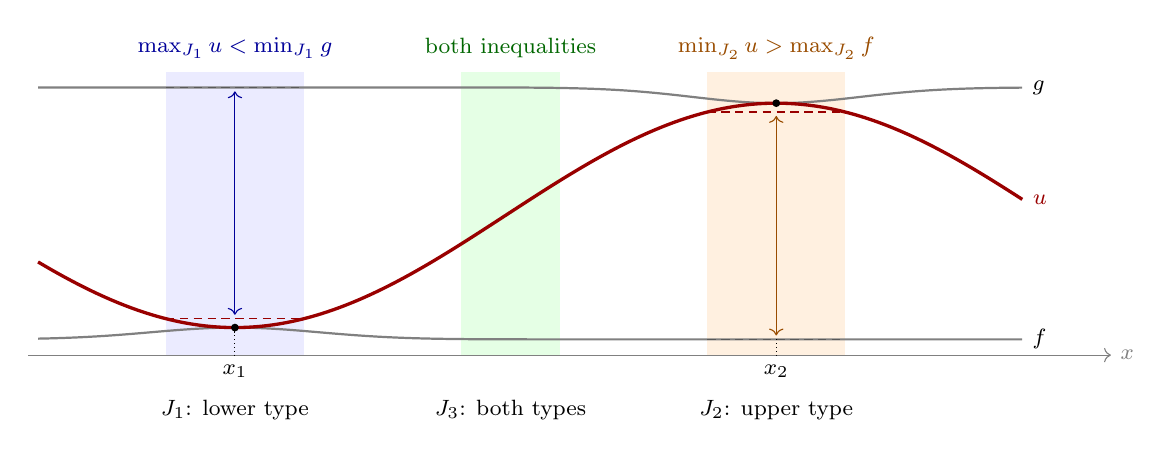
\begin{tikzpicture}[x=1.25cm, y=1cm, font=\footnotesize,
  declare function={F(\t)=0.2+0.15*exp(-((\t-2)/1.2)^2);
    G(\t)=3.4-0.2*exp(-((\t-7.5)/1.2)^2);
    U(\t)=1.775-1.425*cos(deg(pi*(\t-2)/5.5));}]
  % strips
  \fill[blue!8] (1.3,0) rectangle (2.7,3.6);
  \fill[green!10] (4.3,0) rectangle (5.3,3.6);
  \fill[orange!12] (6.8,0) rectangle (8.2,3.6);
  % axis
  \draw[->, gray] (-0.1,0) -- (10.9,0) node[right] {$x$};
  % obstacles and solution
  \draw[thick, gray, domain=0:10, samples=100, smooth] plot (\x,{F(\x)}) node[right, black] {$f$};
  \draw[thick, gray, domain=0:10, samples=100, smooth] plot (\x,{G(\x)}) node[right, black] {$g$};
  \draw[very thick, red!60!black, domain=0:10, samples=120, smooth] plot (\x,{U(\x)}) node[right] {$u$};
  % J1: lower type
  \draw[densely dashed, red!60!black] (1.3,{U(1.3)}) -- (2.7,{U(1.3)});
  \draw[densely dashed, gray!70!black] (1.3,{G(1.3)}) -- (2.7,{G(1.3)});
  \draw[<->, blue!60!black] (2.0,{U(1.3)+0.05}) -- (2.0,{G(1.3)-0.05});
  \fill (2,0.35) circle (1.4pt);
  \draw[densely dotted] (2,0.35) -- (2,0) node[below] {$x_1$};
  \node[blue!60!black] at (2,3.9) {$\max_{J_1}u<\min_{J_1}g$};
  % J2: upper type
  \draw[densely dashed, red!60!black] (6.8,{U(6.8)}) -- (8.2,{U(6.8)});
  \draw[densely dashed, gray!70!black] (6.8,{F(6.8)}) -- (8.2,{F(6.8)});
  \draw[<->, orange!60!black] (7.5,{F(6.8)+0.05}) -- (7.5,{U(6.8)-0.05});
  \fill (7.5,3.2) circle (1.4pt);
  \draw[densely dotted] (7.5,0.2) -- (7.5,0) node[below] {$x_2$};
  \node[orange!60!black] at (7.5,3.9) {$\min_{J_2}u>\max_{J_2}f$};
  \node[green!40!black] at (4.8,3.9) {both inequalities};
  % labels
  \node[align=center] at (2,-0.7) {$J_1$: lower type};
  \node[align=center] at (4.8,-0.7) {$J_3$: both types};
  \node[align=center] at (7.5,-0.7) {$J_2$: upper type};
\end{tikzpicture}}


\end{document}
